

\section{Experiments}\label{ref:exp}
In this section, we evaluate our proposed \sketrag framework by addressing the following research questions:
\begin{itemize}[topsep=2pt,itemsep=1pt,parsep=0pt,partopsep=0pt,leftmargin=11pt]
\item \textbf{RQ1}: How does \sketrag enhance effectiveness while reducing costs compared to existing solutions?
\item \textbf{RQ2}: What is the contribution of each core subroutine to \sketrag's overall performance?
\item \textbf{RQ3}: How does \sketrag balance result quality, index construction cost, and the trade-off between its two retrieval channels?
\item \textbf{RQ4}: How sensitive is \sketrag's performance to its parameter settings?
\end{itemize}
All experiments are conducted on a Linux machine with Intel Xeon(R) Gold 6240@2.60GHz CPU and 32GB RAM\eat{ in single-thread mode}. We use the OpenAI API to access LLMs.

% \begin{table}[!t]
% \centering
% \caption{Dataset statistics.}\label{tab:dataset-stat}
% \vspace{-3mm}
% \renewcommand{\arraystretch}{1.2}
% \begin{small}
% \begin{tabular}{cccc}
% \toprule
% \textbf{Dataset}     & \textbf{\#hops} & \textbf{\#paragraphs} & \textbf{\#tokens}\\ 
% \midrule 
% MuSiQue & 2, 3, 4 & 6,761 & 751,784\\
% HotpotQA & 2 & 20,150 & 618,325\\
% \bottomrule
% \end{tabular}
% \end{small}
% \end{table}

\begin{table*}[h]
\centering
\renewcommand{\arraystretch}{1.1}
% \begin{small}
\caption{Overall Performance of RAG Methods. Results are reported in low/high-performance versions. The best and second-best results in each column are highlighted in bold and underlined, respectively.}
\label{tab:quality-all}
% \begin{tabular}{lcccc|cccc|cccc}	
%     \toprule
%     \bf Dataset & \multicolumn{4}{c}{\bf MuSiQue} & \multicolumn{4}{c}{\bf 2Wiki} & \multicolumn{4}{c}{\bf HotpotQA} \\
%     \cmidrule(lr){2-5} \cmidrule(lr){6-9} \cmidrule(lr){10-13}
%     \bf Metric & \bf USD & \bf Coverage & \bf EM & \bf F1 & \bf USD & \bf Coverage & \bf EM & \bf F1 & \bf USD & \bf Coverage & \bf EM & \bf F1 \\
%     \toprule
%     \textrag & 0.02/0.05 & 26.4/76.8 & 3.0/12.8 & 5.4/19.4 & 0.01/0.02 & 61.2/66.4 & 17.0/20.6 & 21.5/25.9 & 0.01/0.04 & 37.2/74.0 & 16.0/33.6 & 21.1/44.2 \\
%     \keyrag & 0.03/0.09 & 50.8/78.2 & 7.0/14.6 & 11.8/20.6 & 0.02/0.04 & 69.8/71.8 & 17.0/22.2 & 22.1/28.3 & 0.03/0.07 & 60.2/82.2 & 24.4/33.8 & 33.5/46.4 \\
%     \midrule
%     \knnrag & 0.02/0.05 & & & & 0.01/0.02 & & & & 0.01/0.04 \\
%     \kgrag & 2.30/24.94 & 47.6/69.6 & 11.4/17.4 & 15.8/25.1 & 1.21/12.79 & 54.2/69.0 & 17.4/25.2 & 20.2/30.8 & 2.30/21.29 & 63.0/74.6 & 21.6/31.0 & 30.2/43.0 \\
%     \skeletonragu & 1.86/19.95 & 42.0/71.0 & 10.2/17.4 & 14.1/24.6 & 0.97/10.23 & 49.2/69.2 & 12.8/23.8 & 15.1/30.1 & 1.84/17.03 & 56.4/73.6 & 19.6/32.0 & 27.5/43.0 \\
%     \skeletonragp & 1.86/19.95 & 43.4/69.6 & 11.0/17.4 & 14.1/24.6 & 0.97/10.23 & 50.6/68.8 & 13.8/23.6 & 15.5/29.5 & 1.84/17.03 & -- & -- & -- \\
%     \midrule
%     \hybridrag & 2.32/24.99 & 49.2/80.0 & 10.4/19.4 & 15.1/26.2 & 1.22/12.81 & 67.2/73.2 & 18.6/26.8 & 22.6/32.9 & 2.31/21.33 & 64.8/80.2 & 22.6/34.0 & 30.5/46.1 \\
%     \sketragu & 1.89/20.04 & 76.2/80.2 & 13.4/18.4 & 18.1/25.9 & 0.99/10.27 & 72.4/75.6 & 14.8/26.4 & 18.6/32.1 & 1.87/17.10 & 81.4/82.6 & 28.4/34.8 & 38.2/47.2 \\
%     \sketragp & 1.89/20.04 & 56.8/79.6 & 12.4/19.2 & 17.1/26.6 & 0.99/10.27 & 72.6/75.4 & 15.0/25.8 & 19.4/31.4 & 1.87/17.10 & 66.6/82.6 & 26.1/35.2 & 34.8/47.7 \\
%     \bottomrule
% \end{tabular}
\begin{tabular}{lcccc|cccc}	
    \toprule
    \bf Dataset & \multicolumn{4}{c}{\bf MuSiQue} & \multicolumn{4}{c}{\bf HotpotQA} \\
    \cmidrule(lr){2-5} \cmidrule(lr){6-9}
    \bf Metric & \bf USD & \bf Coverage & \bf EM & \bf F1 & \bf USD & \bf Coverage & \bf EM & \bf F1 \\
    \toprule
\textrag      & 0.02 / 0.05  & 26.4 / 76.8             & 3.0 / 12.8              & 5.4 / 19.4              & 0.01 / 0.04  & 37.2 / 74.0             & 16.0 / 33.6             & 21.1 / 44.2             \\
\knnrag       & 0.02 / 0.05  & 21.2 / 66.0 & 2.8 / 11.2 & 4.6 / 17.5 & 0.01 / 0.04  & 28.6 / 63.2 & 13.4 / 29.8 & 16.9 / 39.6\\
\kgrag     & 2.30 / 24.94 & 47.6 / 69.6             & 11.4 / 17.4             & 15.8 / 25.1             & 2.30 / 21.29 & 63.0 / 74.6             & 21.6 / 31.0             & 30.2 / 43.0             \\
\hybridrag    & 2.32 / 24.99 & 49.2 / {\ul 80.0}       & 10.4 / {\bf 19.4}       & 15.1 / {\ul 26.2}             & 2.31 / 21.33 & 64.8 / 80.2             & 22.6 / 34.0             & 30.5 / 46.1             \\ \midrule
\keyrag       & 0.03 / 0.09  & 50.8 / 78.2             & 7.0 / 14.6              & 11.8 / 20.6             & 0.03 / 0.07  & 60.2 / 82.2             & 24.4 / 33.8             & 33.5 / 46.4             \\
% \skeletonragu & 1.86 / 19.95 & 42.0 / 71.0             & 10.2 / 17.4             & 14.1 / 24.6             & 1.84 / 17.03 & 56.4 / 73.6             & 19.6 / 32.0             & 27.5 / 43.0             \\
\skeletonrag & 1.86 / 19.95 & 43.4 / 69.6             & 11.0 / 17.4             & 14.1 / 24.6             & 1.84 / 17.03 & 57.8 / 74.6 & 20.0 / 31.2                    & 26.7 / 42.8                    \\
\sketragu     & 1.89 / 20.04 & {\ul 76.2} / {\bf 80.2} & {\ul 13.4} / 18.4       & {\ul 18.1} / 25.9 & 1.87 / 17.10 & {\ul 81.4} / {\ul 82.6} & {\ul 28.4} / {\ul 34.8} & {\ul 38.2} / {\ul 47.2} \\
\sketragp     & 1.89 / 20.04 & {\bf 77.0} / 79.6       & {\bf 14.0} / {\ul 19.2} & {\bf 18.9} / {\bf 26.6} & 1.87 / 17.10 & {\bf 81.6} / {\bf 82.6} & {\bf 28.6} / {\bf 35.2} & {\bf 38.7} / {\bf 47.7} \\
    \bottomrule
\end{tabular}
% \end{small}
\end{table*}



\subsection{Experimental Settings}\label{sec:exp-set}

\stitle{Datasets and metrics}
We use two widely adopted benchmarking datasets for multi-hop QA tasks: MuSiQue~\cite{trivedi2022musique} and HotpotQA~\cite{yang2018hotpotqa}. These datasets consist of QA pairs, each accompanied by multiple paragraphs as potential relevant context. Specifically, in MuSiQue, each QA pair is associated with 2 golden paragraphs and 20 candidate paragraphs, while in HotpotQA, each pair includes 8 distracting paragraphs.
Following prior work~\cite{wang2024knowledge, gutierrez2024hipporag}, we sample 500 QA instances from each dataset. The number of question hops is ${2,3,4}$ in MuSiQue and 2 in HotpotQA. The corresponding paragraphs for all sampled instances are preprocessed into $\Tset$ and compiled as the external corpus for RAG~\cite{gutierrez2024hipporag}.
For MuSiQue and HotpotQA, the number of preprocessed paragraphs is 6,761 and 20,150, respectively, resulting in an overall token count of 751,784 and 618,325.
\eat{The number of question hops, the number of original paragraphs processed into text chunks, and the total token count are summarized in Table~\ref{tab:dataset-stat}.}For evaluation, we measure indexing cost by USD, retrieval quality by Coverage, and generation quality using Exact Match (EM) and F1-Score. Coverage is defined as the proportion of the cases that ground-truth answers found within the retrieved context across all QA instances.
To assess generation performance, we use the pre-defined LLM to generate answers by \textit{solely} based on the retrieved context and evaluate them using well-adopted EM and F1-score~\cite{gutierrez2024hipporag,wang2024knowledge,li2024graph}. EM measures the percentage of answers that exactly match the ground truth, while the F1-score quantifies partial correctness by evaluating word-level overlap between predicted and ground-truth answers, balancing precision and recall.

\stitle{Solutions and configurations}
We evaluate the performance of 8 solutions categorized as follows: (i) \textit{Existing competitors}: \textrag~\cite{lewis2020retrieval}, \knnrag~\cite{wang2024knowledge}, \kgrag~\cite{edge2024local}, \hybridrag~\cite{sarmah2024hybridrag}. (ii) \textit{Proposed baselines}: \keyrag, which constructs only $\G_k$ as the index and retrieves from it; \skeletonrag, which retains only $\G_s$. (iii) \textit{Final solutions}: \sketragu and \sketragp, where \textsf{U} and \textsf{P} represent selecting core chunks randomly and via PageRank, respectively. For a fair comparison, we implement existing solutions within the \sketrag framework, demonstrating that our approach serves as a unified and generalized RAG framework. Specifically, for \textrag and \knnrag, we use the KNN graph constructed in Algorithm~\ref{alg:sketrag-index} as the index $\G$. \sketrag reduces to \textrag when retrieving only the seed nodes in $\G$ and to \knnrag when also including their neighbors. Furthermore, \sketrag simplifies to \kgrag by setting $\beta=1$ and $\theta=1$ and to \hybridrag by combining both \textrag and \kgrag. Notably, \hybridrag fully constructs indices for both \textrag and \kgrag, retrieving content equally from both. This setup effectively corresponds to $\beta=0.5$ under a fixed context limit. 
Regarding the base models in each solution, we use OpenAI's \texttt{GPT-4o-mini} as the LLM for inference, OpenAI's \texttt{text-embedding-3-small} for text embedding generation, \texttt{cl100k\_base} for word tokenization, and the \texttt{sent\_tokenize} function from the \texttt{nltk} Python library for sentence tokenization.
We follow the default settings in~\citet{edge2024local}, setting the input chunk size $\ell$ to 1,200 and the output context limit $\lambda$ to 12,000 across all solutions. Within \sketrag, we use the default parameters for components related to \kgrag and set $K=2$, $\beta=0.8$, and $\theta=0.4$, unless specified otherwise.
The implementations of all solutions are available at {\color{blue}\url{https://github.com/waetr/KET-RAG}}.
% https://anonymous.4open.science/r/KET-RAG-FC06/

\subsection{Performance Evaluation (RQ1)}
In the first set of experiments, we evaluate the performance of \sketrag against existing competitors (\textrag, \knnrag, \kgrag, and \hybridrag) under two configurations: a low-cost version with reduced accuracy and a high-accuracy version with increased cost. Following previous works~\cite{edge2024local}, we achieve the low-cost setting by using an input chunk size of $\ell = 1,200$ and the high-accuracy setting by fixing $\ell = 150$ for all solutions. For \keyrag and \sketrag, we set $\tau$ to 3 and 0, respectively, ensuring the same text sub-chunk length in both configurations.

As reported in Table \ref{tab:quality-all}, our proposed \sketrag(\textsf{-U}/\textsf{-P}) achieves superior quality-cost trade-offs compared to existing methods on both MuSiQue and HotpotQA.
In terms of retrieval quality, \sketrag significantly outperforms all baselines, achieving the coverage score of 77.0\%/80.2\% and 81.6\%/82.6\% on MuSiQue and HotpotQA, respectively. Compared to the best competitor \hybridrag, this corresponds to relative improvements of 56.5\% and 25.9\% on MuSiQue and HotpotQA, respectively. Most notably, we observe that \sketrag in low-cost mode achieves comparable or even superior coverage to \kgrag and \hybridrag in high-accuracy mode while reducing indexing costs by over an order of magnitude. For example, on HotpotQA, the coverage scores of \sketragp, \hybridrag, and \kgrag are 81.6\%, 80.2\%, and 74.6\%, respectively, yet \sketragp incurs only 8.7\% of their indexing cost.
Akin to the retrieval quality, \sketrag achieves competitive generation quality at lower costs. Take the low-cost mode as an example. It improves \hybridrag by 34.6\%/25.2\% (resp.\ 26.5\%/26.9\%) in EM/F1 scores on MuSiQue (resp.\ HotpotQA) while reducing indexing costs by $19\%$.

Regarding other competitors, we observe that \textrag exhibits a more pronounced accuracy improvement compared to \kgrag when transitioning from low- to high-accuracy mode, which motivates the text splitting strategy in \sketrag.
Additionally, we find that, on HotpotQA, the generation quality of \kgrag is slightly lower than that of \textrag in the high-accuracy setting. This is because HotPotQA is a weaker benchmark for multi-hop reasoning due to the presence of spurious signals~\cite{gutierrez2024hipporag, trivedi2022musique}. Despite this, \sketrag consistently outperforms both competitors, demonstrating its robustness across different knowledge retrieval scenarios.



\begin{figure}[t]
\centering
\begin{tikzpicture}
    \begin{customlegend}[legend columns=4,
        legend entries={\sketragp, \sketragu, \skeletonrag\eat{, \skeletonragu}}
        ,
        legend style={at={(0.45,1.05)},anchor=north,draw=none,font=\footnotesize,column sep=0.1cm}]
    \addlegendimage{line width=0.3mm,mark size=2pt,mark=o,color=Red}
    \addlegendimage{line width=0.3mm,mark size=2pt,mark=x,color=Orange}
    \addlegendimage{line width=0.3mm,mark size=2pt,mark=triangle,color=LightBlue}
    % \addlegendimage{line width=0.3mm,mark size=2pt,mark=star,color=DeepBlue}
    \end{customlegend}
\end{tikzpicture}
% \vspace{-2mm}
\\
\subfloat[MuSiQue]{
\hspace{-1.2mm}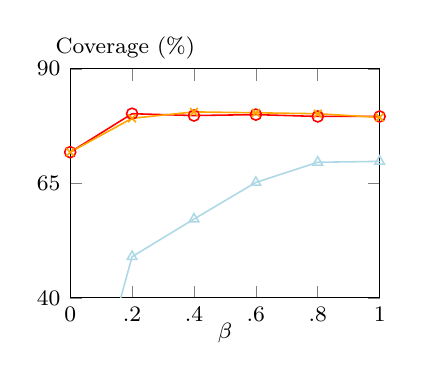
\begin{tikzpicture}[scale=1]
    \begin{axis}[
        height=\columnwidth/2.7,
        width=\columnwidth/2.2,
        ylabel={Coverage (\%)},
        xlabel={$\beta$},
        xmin=0.0, xmax=1.0,
        ymin=0.4, ymax=0.9,
        xtick={0, 0.2, 0.4, 0.6, 0.8, 1.0},
        xticklabel style = {font=\footnotesize},
        xticklabels={0, .2, .4, .6, .8, 1},
        ytick={0.4, 0.65, 0.9},
        yticklabels={40, 65, 90},
        every axis y label/.style={at={(current axis.north west)},right=7mm,above=0mm},
        label style={font=\footnotesize},
        tick label style={font=\footnotesize},
        every axis x label/.style={at={(current axis.south)},right=0mm,above=-7mm},
        label style={font=\footnotesize},
        tick label style={font=\footnotesize},
    ]

%     \addplot[line width=0.2mm,mark size=2pt,mark=o,color=Red]
%         plot coordinates { % SkeTRAG - 1200
% (0, 0.176300934)
% (0.2, 0.188094157)
% (0.4, 0.196128801)
% (0.6, 0.1876783)
% (0.8, 0.19700453)
% (1.0, 0.157561628)
%     };

%     \addplot[line width=0.2mm,mark size=2pt,mark=o,color=Red!75]
%         plot coordinates { % SkeTRAG - 600
% (0, 0.170179462)
% (0.2, 0.240968426)
% (0.4, 0.226319961)
% (0.6, 0.232188549)
% (0.8, 0.229216351)
% (1.0, 0.208775333)
%     };

%     \addplot[line width=0.2mm,mark size=2pt,mark=o,color=Red!50]
%         plot coordinates { % SkeTRAG - 300
% (0, 0.169292118)
% (0.2, 0.24154141)
% (0.4, 0.256892671)
% (0.6, 0.255549124)
% (0.8, 0.266975679)
% (1.0, 0.256770818)
%     };

    \addplot[line width=0.2mm,mark size=2pt,mark=o,color=Red]
        plot coordinates { % SkeTRAG - 150
(0.0, 0.718)
(0.2, 0.802)
(0.4, 0.798)
(0.6, 0.8)
(0.8, 0.796)
(1.0, 0.796)
    };

    \addplot[line width=0.2mm,mark size=2pt,mark=x,color=Orange]
        plot coordinates { % SkeTRAG - uniform
(0.0, 0.718)
(0.2, 0.792)
(0.4, 0.806)
(0.6, 0.804)
(0.8, 0.802)
(1.0, 0.794)
    };

    \addplot[line width=0.2mm,mark size=2pt,mark=triangle,color=LightBlue]
        plot coordinates { % skeleton
(0.0, 0.0)
(0.2, 0.49)
(0.4, 0.572)
(0.6, 0.652)
(0.8, 0.696)
(1.0, 0.698)
    };

%     \addplot[line width=0.2mm,mark size=2pt,mark=star,color=DeepBlue]
%         plot coordinates { % skeleton - uniform
% (0.0, 0.0)
% (0.2, 0.462)
% (0.4, 0.62)
% (0.6, 0.694)
% (0.8, 0.71)
% (1.0, 0.696)
%     };

\end{axis}

\end{tikzpicture}
\hspace{-1.2mm}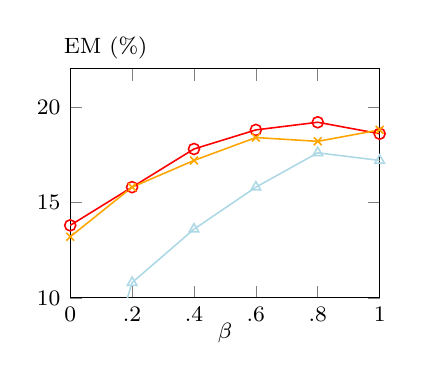
\begin{tikzpicture}[scale=1]
    \begin{axis}[
        height=\columnwidth/2.7,
        width=\columnwidth/2.2,
        ylabel={EM (\%)},
        xlabel={$\beta$},
        xmin=0.0, xmax=1.0,
        ymin=0.1, ymax=0.22,
        xtick={0, 0.2, 0.4, 0.6, 0.8, 1.0},
        xticklabel style = {font=\footnotesize},
        xticklabels={0, .2, .4, .6, .8, 1},
        ytick={0.1, 0.15, 0.2},
        yticklabels={10, 15, 20},
        every axis y label/.style={at={(current axis.north west)},right=4.5mm,above=0mm},
        label style={font=\footnotesize},
        tick label style={font=\footnotesize},
        every axis x label/.style={at={(current axis.south)},right=0mm,above=-7mm},
        label style={font=\footnotesize},
        tick label style={font=\footnotesize},
    ]

%     \addplot[line width=0.2mm,mark size=2pt,mark=o,color=Red]
%         plot coordinates { % SkeTRAG
% (0, 0.122)
% (0.2, 0.132)
% (0.4, 0.144)
% (0.6, 0.134)
% (0.8, 0.14)
% (1.0, 0.114)
%     };

%     \addplot[line width=0.2mm,mark size=2pt,mark=o,color=Red!75]
%         plot coordinates { % SkeTRAG - 600
% (0, 0.108)
% (0.2, 0.174)
% (0.4, 0.17)
% (0.6, 0.172)
% (0.8, 0.166)
% (1.0, 0.152)
%     };

%     \addplot[line width=0.2mm,mark size=2pt,mark=o,color=Red!50]
%         plot coordinates { % SkeTRAG - 300
% (0, 0.104)
% (0.2, 0.176)
% (0.4, 0.192)
% (0.6, 0.186)
% (0.8, 0.198)
% (1.0, 0.192)
%     };

    \addplot[line width=0.2mm,mark size=2pt,mark=o,color=Red]
        plot coordinates { % SkeTRAG - 150
(0.0, 0.138)
(0.2, 0.158)
(0.4, 0.178)
(0.6, 0.188)
(0.8, 0.192)
(1.0, 0.186)
    };

    \addplot[line width=0.2mm,mark size=2pt,mark=x,color=Orange]
        plot coordinates { % SkeTRAG - uniform
(0.0, 0.132)
(0.2, 0.158)
(0.4, 0.172)
(0.6, 0.184)
(0.8, 0.182)
(1.0, 0.188)
    };

%     \addplot[line width=0.2mm,mark size=2pt,mark=star,color=DeepBlue]
%         plot coordinates { % skeleton - uniform
% (0.0, 0.0)
% (0.2, 0.106)
% (0.4, 0.132)
% (0.6, 0.164)
% (0.8, 0.174)
% (1.0, 0.174)
%     };


    \addplot[line width=0.2mm,mark size=2pt,mark=triangle,color=LightBlue]
        plot coordinates { % skeleton
(0.0, 0.0)
(0.2, 0.108)
(0.4, 0.136)
(0.6, 0.158)
(0.8, 0.176)
(1.0, 0.172)
    };
    
    \end{axis}

\end{tikzpicture}
\hspace{-1.2mm}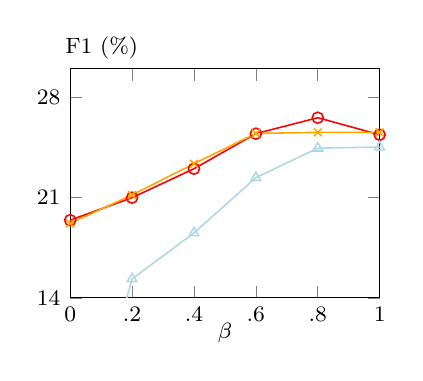
\begin{tikzpicture}[scale=1]
    \begin{axis}[
        height=\columnwidth/2.7,
        width=\columnwidth/2.2,
        ylabel={F1 (\%)},
        xlabel={$\beta$},
        xmin=0.0, xmax=1.0,
        ymin=0.14, ymax=0.3,
        xtick={0, 0.2, 0.4, 0.6, 0.8, 1.0},
        xticklabel style = {font=\footnotesize},
        xticklabels={0, .2, .4, .6, .8, 1},
        ytick={0.14, 0.21, 0.28},
        yticklabels={14, 21, 28},
        every axis y label/.style={at={(current axis.north west)},right=4mm,above=0mm},
        label style={font=\footnotesize},
        tick label style={font=\footnotesize},
        every axis x label/.style={at={(current axis.south)},right=0mm,above=-7mm},
        label style={font=\footnotesize},
        tick label style={font=\footnotesize},
    ]

%     \addplot[line width=0.2mm,mark size=2pt,mark=o,color=Red]
%         plot coordinates { % SkeTRAG - 1200
% (0, 0.176300934)
% (0.2, 0.188094157)
% (0.4, 0.196128801)
% (0.6, 0.1876783)
% (0.8, 0.19700453)
% (1.0, 0.157561628)
%     };

%     \addplot[line width=0.2mm,mark size=2pt,mark=o,color=Red!75]
%         plot coordinates { % SkeTRAG - 600
% (0, 0.170179462)
% (0.2, 0.240968426)
% (0.4, 0.226319961)
% (0.6, 0.232188549)
% (0.8, 0.229216351)
% (1.0, 0.208775333)
%     };

%     \addplot[line width=0.2mm,mark size=2pt,mark=o,color=Red!50]
%         plot coordinates { % SkeTRAG - 300
% (0, 0.169292118)
% (0.2, 0.24154141)
% (0.4, 0.256892671)
% (0.6, 0.255549124)
% (0.8, 0.266975679)
% (1.0, 0.256770818)
%     };

    \addplot[line width=0.2mm,mark size=2pt,mark=o,color=Red]
        plot coordinates { % SkeTRAG - 150
(0.0, 0.194302287)
(0.2, 0.209992062)
(0.4, 0.23021343)
(0.6, 0.254704947)
(0.8, 0.265845586)
(1.0, 0.253952005)
    };

    \addplot[line width=0.2mm,mark size=2pt,mark=x,color=Orange]
        plot coordinates { % SkeTRAG - uniform
(0.0, 0.192066627)
(0.2, 0.211880355)
(0.4, 0.233691958)
(0.6, 0.254856333)
(0.8, 0.255602241)
(1.0, 0.255616111)
    };

    \addplot[line width=0.2mm,mark size=2pt,mark=triangle,color=LightBlue]
        plot coordinates { % skeleton
(0.0, 0.0)
(0.2, 0.153266376)
(0.4, 0.185392483)
(0.6, 0.223946198)
(0.8, 0.244550107)
(1.0, 0.245370649)
    };

%     \addplot[line width=0.2mm,mark size=2pt,mark=star,color=DeepBlue]
%         plot coordinates { % skeleton - uniform
% (0.0, 0.0)
% (0.2, 0.148484271)
% (0.4, 0.200356146)
% (0.6, 0.235926157)
% (0.8, 0.247588566)
% (1.0, 0.247293046)
%     };

\end{axis}

\end{tikzpicture}
}%
\\
\subfloat[Hotpot]{
\hspace{-1.2mm}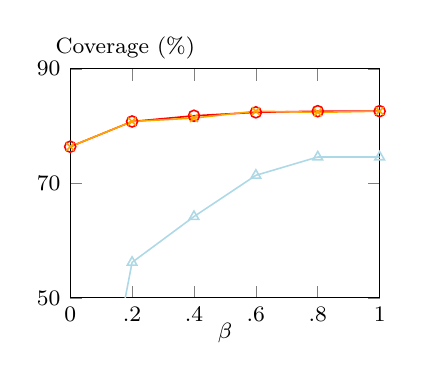
\begin{tikzpicture}[scale=1]
    \begin{axis}[
        height=\columnwidth/2.7,
        width=\columnwidth/2.2,
        ylabel={Coverage (\%)},
        xlabel={$\beta$},
        xmin=0.0, xmax=1.0,
        ymin=0.5, ymax=0.9,
        xtick={0, 0.2, 0.4, 0.6, 0.8, 1.0},
        xticklabel style = {font=\footnotesize},
        xticklabels={0, .2, .4, .6, .8, 1},
        ytick={0.5, 0.7, 0.9},
        yticklabels={50, 70, 90},
        every axis y label/.style={at={(current axis.north west)},right=7mm,above=0mm},
        label style={font=\footnotesize},
        tick label style={font=\footnotesize},
        every axis x label/.style={at={(current axis.south)},right=0mm,above=-7mm},
        label style={font=\footnotesize},
        tick label style={font=\footnotesize},
    ]

    \addplot[line width=0.2mm,mark size=2pt,mark=o,color=Red]
        plot coordinates { % SkeTRAG - 150
(0.0, 0.764)
(0.2, 0.808)
(0.4, 0.818)
(0.6, 0.824)
(0.8, 0.826)
(1.0, 0.826)
    };

    \addplot[line width=0.2mm,mark size=2pt,mark=x,color=Orange]
        plot coordinates { % SkeTRAG - uniform
(0.0, 0.764)
(0.2, 0.808)
(0.4, 0.814)
(0.6, 0.826)
(0.8, 0.824)
(1.0, 0.826)
    };

    \addplot[line width=0.2mm,mark size=2pt,mark=triangle,color=LightBlue]
        plot coordinates { % skeleton
(0.0, 0.0)
(0.2, 0.562)
(0.4, 0.642)
(0.6, 0.714)
(0.8, 0.746)
(1.0, 0.746)
    };

%     \addplot[line width=0.2mm,mark size=2pt,mark=star,color=DeepBlue]
%         plot coordinates { % skeleton - uniform
% (0.0, 0.0)
% (0.2, 0.576)
% (0.4, 0.686)
% (0.6, 0.732)
% (0.8, 0.736)
% (1.0, 0.746)
%     };
    \end{axis}

\end{tikzpicture}
\hspace{-1.2mm}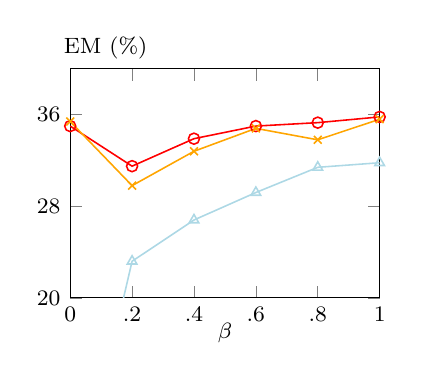
\begin{tikzpicture}[scale=1]
    \begin{axis}[
        height=\columnwidth/2.7,
        width=\columnwidth/2.2,
        ylabel={EM (\%)},
        xlabel={$\beta$},
        xmin=0.0, xmax=1.0,
        ymin=0.2, ymax=0.4,
        xtick={0, 0.2, 0.4, 0.6, 0.8, 1.0},
        xticklabel style = {font=\footnotesize},
        xticklabels={0, .2, .4, .6, .8, 1},
        ytick={0.2, 0.28, 0.36},
        yticklabels={20, 28, 36},
        every axis y label/.style={at={(current axis.north west)},right=4.5mm,above=0mm},
        label style={font=\footnotesize},
        tick label style={font=\footnotesize},
        every axis x label/.style={at={(current axis.south)},right=0mm,above=-7mm},
        label style={font=\footnotesize},
        tick label style={font=\footnotesize},
    ]

    \addplot[line width=0.2mm,mark size=2pt,mark=o,color=Red]
        plot coordinates { % SkeTRAG - 150
(0.0, 0.35)
(0.2, 0.315)
(0.4, 0.339)
(0.6, 0.35)
(0.8, 0.353)
(1.0, 0.358)
    };

    \addplot[line width=0.2mm,mark size=2pt,mark=x,color=Orange]
        plot coordinates { % SkeTRAG - uniform
(0.0, 0.354)
(0.2, 0.298)
(0.4, 0.328)
(0.6, 0.348)
(0.8, 0.338)
(1.0, 0.356)
    };

    \addplot[line width=0.2mm,mark size=2pt,mark=triangle,color=LightBlue]
        plot coordinates { % skeleton
(0.0, 0.0)
(0.2, 0.232)
(0.4, 0.268)
(0.6, 0.292)
(0.8, 0.314)
(1.0, 0.318)
    };

%     \addplot[line width=0.2mm,mark size=2pt,mark=star,color=DeepBlue]
%         plot coordinates { % skeleton - uniform
% (0.0, 0.0)
% (0.2, 0.204)
% (0.4, 0.302)
% (0.6, 0.318)
% (0.8, 0.326)
% (1.0, 0.318)
%     };
    
    \end{axis}

\end{tikzpicture}
\hspace{-1.2mm}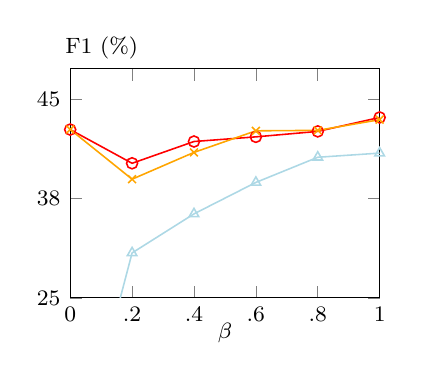
\begin{tikzpicture}[scale=1]
    \begin{axis}[
        height=\columnwidth/2.7,
        width=\columnwidth/2.2,
        ylabel={F1 (\%)},
        xlabel={$\beta$},
        xmin=0.0, xmax=1.0,
        ymin=0.25, ymax=0.55,
        xtick={0, 0.2, 0.4, 0.6, 0.8, 1.0},
        xticklabel style = {font=\footnotesize},
        xticklabels={0, .2, .4, .6, .8, 1},
        ytick={0.25,0.38, 0.51},
        yticklabels={25, 38, 45, 51},
        every axis y label/.style={at={(current axis.north west)},right=4mm,above=0mm},
        label style={font=\footnotesize},
        tick label style={font=\footnotesize},
        every axis x label/.style={at={(current axis.south)},right=0mm,above=-7mm},
        label style={font=\footnotesize},
        tick label style={font=\footnotesize},
    ]

    \addplot[line width=0.2mm,mark size=2pt,mark=o,color=Red]
        plot coordinates { % SkeTRAG - 150
(0.0, 0.470434704)
(0.2, 0.426276111)
(0.4, 0.454788870)
(0.6, 0.460886061)
(0.8, 0.468036694)
(1.0, 0.486306113)
    };

    \addplot[line width=0.2mm,mark size=2pt,mark=x,color=Orange]
        plot coordinates { % SkeTRAG - uniform
(0.0, 0.470574266)
(0.2, 0.405430301)
(0.4, 0.44053814)
(0.6, 0.468784679)
(0.8, 0.469378725)
(1.0, 0.483362192)
    };

    \addplot[line width=0.2mm,mark size=2pt,mark=triangle,color=LightBlue]
        plot coordinates { % skeleton
(0.0, 0.0)
(0.2, 0.308885359)
(0.4, 0.360015033)
(0.6, 0.401194074)
(0.8, 0.434159393)
(1.0, 0.439605784)
    };

%     \addplot[line width=0.2mm,mark size=2pt,mark=star,color=DeepBlue]
%         plot coordinates { % skeleton - uniform
% (0.0, 0.0)
% (0.2, 0.282341829)
% (0.4, 0.394474657)
% (0.6, 0.430782795)
% (0.8, 0.434493561)
% (1.0, 0.438056246)
%     };
    
    \end{axis}

\end{tikzpicture}
}%
\vspace{-2mm}
\caption{Answer quality by varying $\beta$.} \label{fig:quality-beta}
\vspace{-4mm}
\end{figure}

\subsection{Ablation Study (RQ2)}
In the second set of experiments, we evaluate the performance of each single building block proposed in \sketrag, whose results are also included in Table \ref{tab:quality-all}.

\stitle{Knowledge graph skeleton}
We evaluate the performance of \skeletonrag with its full version, \kgrag. By default, \skeletonrag sets $\beta=0.8$, resulting in a 20\% reduction in indexing cost across all cases. 
Surprisingly, we find that \skeletonrag trades off only minor performance reductions, particularly in low-cost settings, while maintaining parity in high-accuracy configurations. For instance, in terms of EM score, \skeletonrag exhibits a relative decrease of 3.5\% and 7.4\% in the low-cost setting on MuSiQue and HotpotQA, respectively. However, in high-accuracy settings, there is no performance drop, and in the case of HotpotQA, even a slight improvement is observed. These results suggest that \skeletonrag effectively balances efficiency and quality, making it a viable alternative to full-scale knowledge graph indexing.

\stitle{Text-keyword bipartite graph}
We compare \keyrag with the conventional \textrag. To ensure a fair comparison, we set $\tau=0$ for \keyrag, allowing both \keyrag and \textrag to retrieve text chunks of the same size. As shown in Table~\ref{tab:quality-all}, \keyrag consistently outperforms \textrag in retrieval and generation quality. Notably, in the low-cost setting, \keyrag achieves 92.4\%/133.3\%/118.5\% and 61.8\%/52.5\%/58.8\% relative improvement in Coverage/EM/F1 on MuSiQue and HotpotQA, respectively, with more significant gains on MuSiQue. These results demonstrate the effectiveness of retrieving context from neighboring text chunks of keyword seeds, particularly in complex multi-hop reasoning.

\stitle{Core text chunk identification}
Based on the results in Table~\ref{tab:quality-all}, we observe that \sketragp shows better quality than \sketragu in both the low-cost and high-cost modes. For instance, \sketragp outperforms \sketragu by up to 1.0\%/4.5\%/4.4\% in Coverage/EM/F1 scores on MuSiQue.
This confirms the effectiveness of the core chunk identification technique, as motivated in Section~\ref{sec:ket-rationale}.
Additionally, we observe that the superiority of \sketragp remains consistent across different settings of $\beta$ and $\theta$, as further illustrated in Figures~\ref{fig:quality-beta}–\ref{fig:quality-theta}.
\eat{This is because larger text chunks in the low-cost setting reduce the accuracy of the constructed KNN graph, leading to less reliable PageRank centrality. More specifically, a larger text chunk inherently acts as an explicit clustering of the smaller consecutive ones within it. However, this ad-hoc clustering is based solely on context adjacency, disregarding lexical and semantic similarities, which affects the effectiveness of PageRank in identifying central nodes.
Additionally, we find that \sketragu and \sketragp exhibit comparable performance in most cases. The advantage of \sketragp becomes more pronounced when only a small set of core chunks are required (\ie $\beta$ and $\theta$ is small). These results are further illustrated in Figures~\ref{fig:quality-beta}-\ref{fig:quality-theta}.}


\begin{figure}[t]
\centering
\begin{tikzpicture}
    \begin{customlegend}[legend columns=3,
        legend entries={\sketragp, \sketragu, \hybridrag}
        ,
        legend style={at={(0.45,1.05)},anchor=north,draw=none,font=\footnotesize,column sep=0.1cm}]
    \addlegendimage{line width=0.3mm,mark size=2pt,mark=o,color=Red}
    \addlegendimage{line width=0.3mm,mark size=2pt,mark=x,color=Orange}
    \addlegendimage{line width=0.3mm,mark size=2pt,mark=pentagon,color=Green}
    \end{customlegend}
\end{tikzpicture}
\\
\subfloat[MuSiQue]{
\hspace{-1.2mm}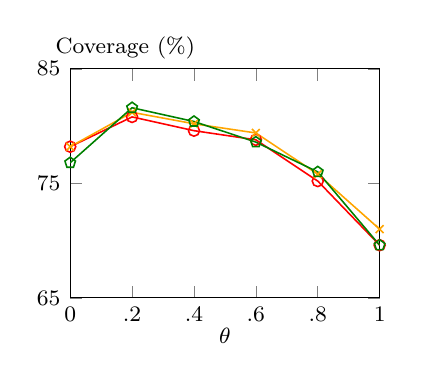
\begin{tikzpicture}[scale=1]
    \begin{axis}[
        height=\columnwidth/2.7,
        width=\columnwidth/2.2,
        ylabel={Coverage (\%)},
        xlabel={$\theta$},
        xmin=0.0, xmax=1.0,
        ymin=0.65, ymax=0.85,
        xtick={0, 0.2, 0.4, 0.6, 0.8, 1.0},
        xticklabel style = {font=\footnotesize},
        xticklabels={0, .2, .4, .6, .8, 1},
        ytick={0.65,0.75,0.85},
        yticklabels={65,75,85},
        every axis y label/.style={at={(current axis.north west)},right=7mm,above=0mm},
        label style={font=\footnotesize},
        tick label style={font=\footnotesize},
        every axis x label/.style={at={(current axis.south)},right=0mm,above=-7mm},
        label style={font=\footnotesize},
        tick label style={font=\footnotesize},
    ]

%     \addplot[line width=0.2mm,mark size=2pt,mark=o,color=Red]
%         plot coordinates { % SkeTRAG - 1200
% (0, 0.176300934)
% (0.2, 0.188094157)
% (0.4, 0.196128801)
% (0.6, 0.1876783)
% (0.8, 0.19700453)
% (1.0, 0.157561628)
%     };

%     \addplot[line width=0.2mm,mark size=2pt,mark=o,color=Red!75]
%         plot coordinates { % SkeTRAG - 600
% (0, 0.170179462)
% (0.2, 0.240968426)
% (0.4, 0.226319961)
% (0.6, 0.232188549)
% (0.8, 0.229216351)
% (1.0, 0.208775333)
%     };

%     \addplot[line width=0.2mm,mark size=2pt,mark=o,color=Red!50]
%         plot coordinates { % SkeTRAG - 300
% (0, 0.169292118)
% (0.2, 0.24154141)
% (0.4, 0.256892671)
% (0.6, 0.255549124)
% (0.8, 0.266975679)
% (1.0, 0.256770818)
%     };

    \addplot[line width=0.2mm,mark size=2pt,mark=o,color=Red]
        plot coordinates { % SkeTRAG - 150
(0.0, 0.782)
(0.2, 0.808)
(0.4, 0.796)
(0.6, 0.788)
(0.8, 0.752)
(1.0, 0.696)
    };

    \addplot[line width=0.2mm,mark size=2pt,mark=x,color=Orange]
        plot coordinates { % SkeTRAG - uniform
(0.0, 0.782)
(0.2, 0.812)
(0.4, 0.802)
(0.6, 0.794)
(0.8, 0.758)
(1.0, 0.71)
    };

    \addplot[line width=0.2mm,mark size=2pt,mark=pentagon,color=Green]
        plot coordinates { % Hybrid
(0.0, 0.768)
(0.2, 0.816)
(0.4, 0.804)
(0.6, 0.786)
(0.8, 0.76)
(1.0, 0.696)
    };



\end{axis}

\end{tikzpicture}
\hspace{-1.2mm}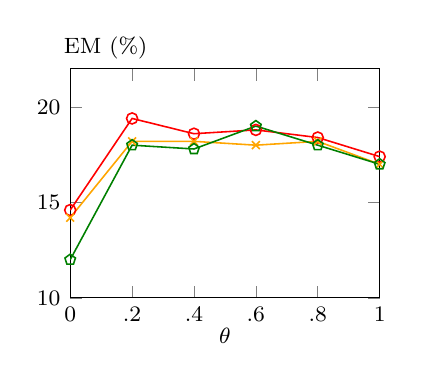
\begin{tikzpicture}[scale=1]
    \begin{axis}[
        height=\columnwidth/2.7,
        width=\columnwidth/2.2,
        ylabel={EM (\%)},
        xlabel={$\theta$},
        xmin=0.0, xmax=1.0,
        ymin=0.1, ymax=0.22,
        xtick={0, 0.2, 0.4, 0.6, 0.8, 1.0},
        xticklabel style = {font=\footnotesize},
        xticklabels={0, .2, .4, .6, .8, 1},
        ytick={0.10, 0.15,0.2},
        yticklabels={10, 15, 20},
        every axis y label/.style={at={(current axis.north west)},right=4.5mm,above=0mm},
        label style={font=\footnotesize},
        tick label style={font=\footnotesize},
        every axis x label/.style={at={(current axis.south)},right=0mm,above=-7mm},
        label style={font=\footnotesize},
        tick label style={font=\footnotesize},
    ]

%     \addplot[line width=0.2mm,mark size=2pt,mark=o,color=Red]
%         plot coordinates { % SkeTRAG
% (0, 0.122)
% (0.2, 0.132)
% (0.4, 0.144)
% (0.6, 0.134)
% (0.8, 0.14)
% (1.0, 0.114)
%     };

%     \addplot[line width=0.2mm,mark size=2pt,mark=o,color=Red!75]
%         plot coordinates { % SkeTRAG - 600
% (0, 0.108)
% (0.2, 0.174)
% (0.4, 0.17)
% (0.6, 0.172)
% (0.8, 0.166)
% (1.0, 0.152)
%     };

%     \addplot[line width=0.2mm,mark size=2pt,mark=o,color=Red!50]
%         plot coordinates { % SkeTRAG - 300
% (0, 0.104)
% (0.2, 0.176)
% (0.4, 0.192)
% (0.6, 0.186)
% (0.8, 0.198)
% (1.0, 0.192)
%     };

    \addplot[line width=0.2mm,mark size=2pt,mark=o,color=Red]
        plot coordinates { % SkeTRAG - 150
(0, 0.146)
(0.2, 0.194)
(0.4, 0.186)
(0.6, 0.188)
(0.8, 0.184)
(1.0, 0.174)
    };

    \addplot[line width=0.2mm,mark size=2pt,mark=x,color=Orange]
        plot coordinates { % SkeTRAG - uniform
(0.0, 0.142)
(0.2, 0.182)
(0.4, 0.182)
(0.6, 0.18)
(0.8, 0.182)
(1.0, 0.17)
    };


    \addplot[line width=0.2mm,mark size=2pt,mark=pentagon,color=Green]
        plot coordinates { % Hybrid
(0.0, 0.12)
(0.2, 0.18)
(0.4, 0.178)
(0.6, 0.19)
(0.8, 0.18)
(1.0, 0.17)
    };
    
    \end{axis}

\end{tikzpicture}
\hspace{-1.2mm}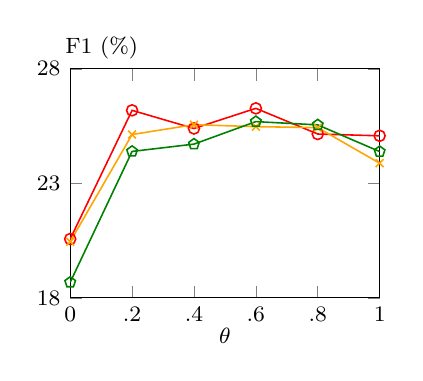
\begin{tikzpicture}[scale=1]
    \begin{axis}[
        height=\columnwidth/2.7,
        width=\columnwidth/2.2,
        ylabel={F1 (\%)},
        xlabel={$\theta$},
        xmin=0.0, xmax=1.0,
        ymin=0.18, ymax=0.28,
        xtick={0, 0.2, 0.4, 0.6, 0.8, 1.0},
        xticklabel style = {font=\footnotesize},
        xticklabels={0, .2, .4, .6, .8, 1},
        ytick={0.18,0.23,0.28},
        yticklabels={18,23,28},
        every axis y label/.style={at={(current axis.north west)},right=4mm,above=0mm},
        label style={font=\footnotesize},
        tick label style={font=\footnotesize},
        every axis x label/.style={at={(current axis.south)},right=0mm,above=-7mm},
        label style={font=\footnotesize},
        tick label style={font=\footnotesize},
    ]

%     \addplot[line width=0.2mm,mark size=2pt,mark=o,color=Red]
%         plot coordinates { % SkeTRAG - 1200
% (0, 0.176300934)
% (0.2, 0.188094157)
% (0.4, 0.196128801)
% (0.6, 0.1876783)
% (0.8, 0.19700453)
% (1.0, 0.157561628)
%     };

%     \addplot[line width=0.2mm,mark size=2pt,mark=o,color=Red!75]
%         plot coordinates { % SkeTRAG - 600
% (0, 0.170179462)
% (0.2, 0.240968426)
% (0.4, 0.226319961)
% (0.6, 0.232188549)
% (0.8, 0.229216351)
% (1.0, 0.208775333)
%     };

%     \addplot[line width=0.2mm,mark size=2pt,mark=o,color=Red!50]
%         plot coordinates { % SkeTRAG - 300
% (0, 0.169292118)
% (0.2, 0.24154141)
% (0.4, 0.256892671)
% (0.6, 0.255549124)
% (0.8, 0.266975679)
% (1.0, 0.256770818)
%     };

    \addplot[line width=0.2mm,mark size=2pt,mark=o,color=Red]
        plot coordinates { % SkeTRAG - 150
(0, 0.205702525)
(0.2, 0.261869012)
(0.4, 0.253952005)
(0.6, 0.262738242)
(0.8, 0.251539304)
(1.0, 0.25075364)
    };

    \addplot[line width=0.2mm,mark size=2pt,mark=x,color=Orange]
        plot coordinates { % SkeTRAG - uniform
(0.0, 0.204517181)
(0.2, 0.251324036)
(0.4, 0.255602241)
(0.6, 0.254754718)
(0.8, 0.254316549)
(1.0, 0.238788916)
    };

    \addplot[line width=0.2mm,mark size=2pt,mark=pentagon,color=Green]
        plot coordinates { % Hybrid
(0.0, 0.186808122)
(0.2, 0.243938036)
(0.4, 0.247127927)
(0.6, 0.256951852)
(0.8, 0.255521173)
(1.0, 0.243875902)
    };

\end{axis}

\end{tikzpicture}
}%
\\
\subfloat[Hotpot]{
\hspace{-1.2mm}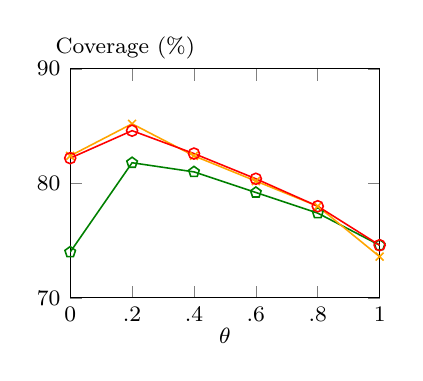
\begin{tikzpicture}[scale=1]
    \begin{axis}[
        height=\columnwidth/2.7,
        width=\columnwidth/2.2,
        ylabel={Coverage (\%)},
        xlabel={$\theta$},
        xmin=0.0, xmax=1.0,
        ymin=0.7, ymax=0.9,
        xtick={0, 0.2, 0.4, 0.6, 0.8, 1.0},
        xticklabel style = {font=\footnotesize},
        xticklabels={0, .2, .4, .6, .8, 1},
        ytick={0.7,0.8,0.9},
        yticklabels={70,80,90},
        every axis y label/.style={at={(current axis.north west)},right=7mm,above=0mm},
        label style={font=\footnotesize},
        tick label style={font=\footnotesize},
        every axis x label/.style={at={(current axis.south)},right=0mm,above=-7mm},
        label style={font=\footnotesize},
        tick label style={font=\footnotesize},
    ]

%     \addplot[line width=0.2mm,mark size=2pt,mark=o,color=Red]
%         plot coordinates { % SkeTRAG - 1200
% (0, 0.413087256)
% (0.2, 0.404018972)
% (0.4, 0.389217444)
% (0.6, 0.389989153)
% (0.8, 0.381677978)
% (1.0, 0.301755047)
%     };

    \addplot[line width=0.2mm,mark size=2pt,mark=pentagon,color=Green]
        plot coordinates { % Hybrid
(0.0, 0.74)
(0.2, 0.818)
(0.4, 0.81)
(0.6, 0.792)
(0.8, 0.774)
(1.0, 0.746)
    };

    \addplot[line width=0.2mm,mark size=2pt,mark=x,color=DeepBlue]
        plot coordinates { % Skeleton

    };

%     \addplot[line width=0.2mm,mark size=2pt,mark=o,color=Red!75]
%         plot coordinates { % SkeTRAG - 600
% (0, 0.412137776)
% (0.2, 0.419856672)
% (0.4, 0.422807675)
% (0.6, 0.437430286)
% (0.8, 0.419080537)
% (1.0, 0.382516896)
%     };

%     \addplot[line width=0.2mm,mark size=2pt,mark=o,color=Red!50]
%         plot coordinates { % SkeTRAG - 300
% (0, 0.437839957)
% (0.2, 0.468297635)
% (0.4, 0.448441971)
% (0.6, 0.443180885)
% (0.8, 0.44557756)
% (1.0, 0.411810544)
%     };

    \addplot[line width=0.2mm,mark size=2pt,mark=x,color=Orange]
        plot coordinates { % SkeTRAG - uniform
(0.0, 0.824)
(0.2, 0.852)
(0.4, 0.824)
(0.6, 0.802)
(0.8, 0.78)
(1.0, 0.736)
    };

    \addplot[line width=0.2mm,mark size=2pt,mark=o,color=Red]
        plot coordinates { % SkeTRAG - 150
(0.0, 0.822)
(0.2, 0.846)
(0.4, 0.826)
(0.6, 0.804)
(0.8, 0.78)
(1.0, 0.746)
    };



    
    \end{axis}

\end{tikzpicture}
\hspace{-1.2mm}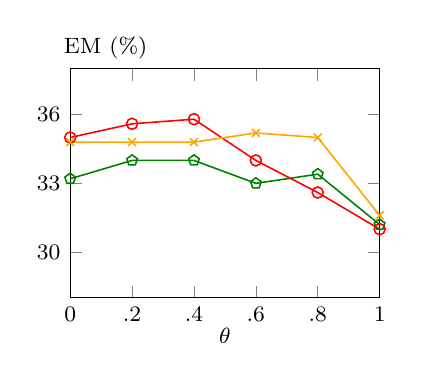
\begin{tikzpicture}[scale=1]
    \begin{axis}[
        height=\columnwidth/2.7,
        width=\columnwidth/2.2,
        ylabel={EM (\%)},
        xlabel={$\theta$},
        xmin=0.0, xmax=1.0,
        ymin=0.28, ymax=0.38,
        xtick={0, 0.2, 0.4, 0.6, 0.8, 1.0},
        xticklabel style = {font=\footnotesize},
        xticklabels={0, .2, .4, .6, .8, 1},
        ytick={0.30, 0.33, 0.36},
        yticklabels={30, 33, 36},
        every axis y label/.style={at={(current axis.north west)},right=4.5mm,above=0mm},
        label style={font=\footnotesize},
        tick label style={font=\footnotesize},
        every axis x label/.style={at={(current axis.south)},right=0mm,above=-7mm},
        label style={font=\footnotesize},
        tick label style={font=\footnotesize},
    ]

%     \addplot[line width=0.2mm,mark size=2pt,mark=o,color=Red]
%         plot coordinates { % SkeTRAG
% (0, 0.298)
% (0.2, 0.296)
% (0.4, 0.288)
% (0.6, 0.288)
% (0.8, 0.282)
% (1.0, 0.216)
%     };

    \addplot[line width=0.2mm,mark size=2pt,mark=pentagon,color=Green]
        plot coordinates { % Hybrid
(0.0, 0.332)
(0.2, 0.34)
(0.4, 0.34)
(0.6, 0.33)
(0.8, 0.334)
(1.0, 0.312)
    };

%     \addplot[line width=0.2mm,mark size=2pt,mark=o,color=Red!75]
%         plot coordinates { % SkeTRAG - 600
% (0, 0.3)
% (0.2, 0.312)
% (0.4, 0.322)
% (0.6, 0.33)
% (0.8, 0.318)
% (1.0, 0.284)
%     };

%     \addplot[line width=0.2mm,mark size=2pt,mark=o,color=Red!50]
%         plot coordinates { % SkeTRAG - 300
% (0, 0.322)
% (0.2, 0.346)
% (0.4, 0.338)
% (0.6, 0.336)
% (0.8, 0.336)
% (1.0, 0.312)
%     };

    \addplot[line width=0.2mm,mark size=2pt,mark=o,color=Red]
        plot coordinates { % SkeTRAG - 150
(0, 0.35)
(0.2, 0.356)
(0.4, 0.358)
(0.6, 0.34)
(0.8, 0.326)
(1.0, 0.31)
    };

    \addplot[line width=0.2mm,mark size=2pt,mark=x,color=Orange]
        plot coordinates { % SkeTRAG - uniform
(0.0, 0.348)
(0.2, 0.348)
(0.4, 0.348)
(0.6, 0.352)
(0.8, 0.350)
(1.0, 0.316)
    };
    
    \end{axis}

\end{tikzpicture}
\hspace{-1.2mm}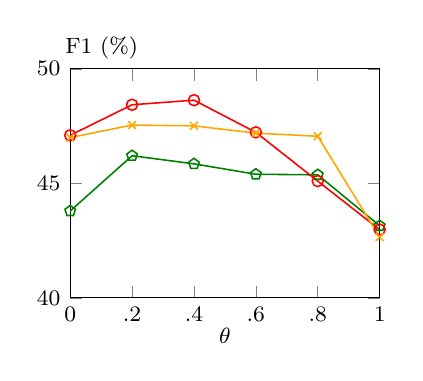
\begin{tikzpicture}[scale=1]
    \begin{axis}[
        height=\columnwidth/2.7,
        width=\columnwidth/2.2,
        ylabel={F1 (\%)},
        xlabel={$\theta$},
        xmin=0.0, xmax=1.0,
        ymin=0.4, ymax=0.5,
        xtick={0, 0.2, 0.4, 0.6, 0.8, 1.0},
        xticklabel style = {font=\footnotesize},
        xticklabels={0, .2, .4, .6, .8, 1},
        ytick={0.4, 0.45, 0.5},
        yticklabels={40, 45, 50},
        every axis y label/.style={at={(current axis.north west)},right=4mm,above=0mm},
        label style={font=\footnotesize},
        tick label style={font=\footnotesize},
        every axis x label/.style={at={(current axis.south)},right=0mm,above=-7mm},
        label style={font=\footnotesize},
        tick label style={font=\footnotesize},
    ]

%     \addplot[line width=0.2mm,mark size=2pt,mark=o,color=Red]
%         plot coordinates { % SkeTRAG - 1200
% (0, 0.413087256)
% (0.2, 0.404018972)
% (0.4, 0.389217444)
% (0.6, 0.389989153)
% (0.8, 0.381677978)
% (1.0, 0.301755047)
%     };

    \addplot[line width=0.2mm,mark size=2pt,mark=pentagon,color=Green]
        plot coordinates { % Hybrid
(0.0, 0.437930177)
(0.2, 0.462061217)
(0.4, 0.458510645)
(0.6, 0.453968044)
(0.8, 0.453729208)
(1.0, 0.431479231)
    };

%     \addplot[line width=0.2mm,mark size=2pt,mark=x,color=DeepBlue]
%         plot coordinates { % Skeleton

%     };

%     \addplot[line width=0.2mm,mark size=2pt,mark=o,color=Red!75]
%         plot coordinates { % SkeTRAG - 600
% (0, 0.412137776)
% (0.2, 0.419856672)
% (0.4, 0.422807675)
% (0.6, 0.437430286)
% (0.8, 0.419080537)
% (1.0, 0.382516896)
%     };

%     \addplot[line width=0.2mm,mark size=2pt,mark=o,color=Red!50]
%         plot coordinates { % SkeTRAG - 300
% (0, 0.437839957)
% (0.2, 0.468297635)
% (0.4, 0.448441971)
% (0.6, 0.443180885)
% (0.8, 0.44557756)
% (1.0, 0.411810544)
%     };

    \addplot[line width=0.2mm,mark size=2pt,mark=o,color=Red]
        plot coordinates { % SkeTRAG - 150
(0, 0.470963143)
(0.2, 0.484303943)
(0.4, 0.486306113)
(0.6, 0.472271351)
(0.8, 0.450982308)
(1.0, 0.429801034)
    };

    \addplot[line width=0.2mm,mark size=2pt,mark=x,color=Orange]
        plot coordinates { % SkeTRAG - uniform
(0.0, 0.469989276)
(0.2, 0.475449933)
(0.4, 0.4751002065)
(0.6, 0.4719215465)
(0.8, 0.4705509015)
(1.0, 0.426568579)
    };


    \end{axis}

\end{tikzpicture}
}%
\vspace{-2mm}
\caption{Answer quality by varying $\theta$.} \label{fig:quality-theta}
\vspace{-2mm}
\end{figure}
% \begin{figure}[h]
\centering
\begin{tikzpicture}
    \begin{customlegend}[legend columns=3,
        legend entries={{SkeTRAG (PageRank)},{(Graph$+$Text)RAG ($\theta=0.2$)}, {TextRAG}}
        ,
        legend style={at={(0.45,1.05)},anchor=north,draw=none,font=\footnotesize,column sep=0.1cm}]
    \addlegendimage{line width=0.3mm,mark size=2pt,mark=o,color=Red}
    \addlegendimage{line width=0.3mm,mark size=2pt,mark=pentagon,color=Green}
    \addlegendimage{line width=0.3mm,mark size=2pt,mark=triangle,color=LightBlue}
    \end{customlegend}
\end{tikzpicture}
\\[-\lineskip]
\subfloat[MuSiQue]{
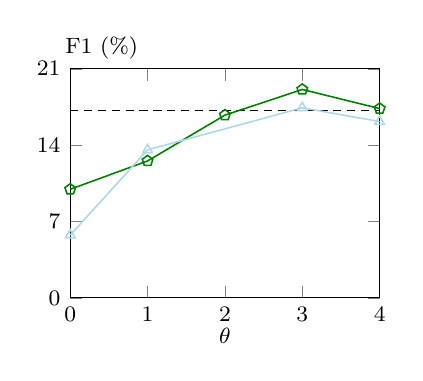
\begin{tikzpicture}[scale=1]
    \begin{axis}[
        height=\columnwidth/2.7,
        width=\columnwidth/2.2,
        ylabel={F1 (\%)},
        xlabel={$\theta$},
        xmin=0, xmax=4,
        ymin=0, ymax=0.21,
        xtick={0,1,2,3,4},
        xticklabel style = {font=\footnotesize},
        xticklabels={0,1,2,3,4},
        ytick={0, 0.07, 0.14, 0.21},
        yticklabels={0, 7, 14, 21},
        every axis y label/.style={at={(current axis.north west)},right=4mm,above=0mm},
        label style={font=\footnotesize},
        tick label style={font=\footnotesize},
        every axis x label/.style={at={(current axis.south)},right=0mm,above=-7mm},
        label style={font=\footnotesize},
        tick label style={font=\footnotesize},
    ]
\addplot[densely dashed, color=black, line width=0.1mm] coordinates {(0, 0.171508414) (4, 0.171508414)};
    \addplot[line width=0.2mm,mark size=2pt,mark=o,color=Red]
        plot coordinates { % SkeTRAG

    };

    \addplot[line width=0.2mm,mark size=2pt,mark=pentagon,color=Green]
        plot coordinates { % Hybrid
(0, 0.099545614)
(1, 0.125519636)
(2, 0.167524344)
(3, 0.191059656)
(4, 0.173562826)
    };

    \addplot[line width=0.2mm,mark size=2pt,mark=triangle,color=LightBlue]
        plot coordinates { % TextRAG
(0, 0.057530199)
(1, 0.135702597)
(3, 0.17426039)
(4, 0.161658265)
    };

    \addplot[line width=0.2mm,mark size=2pt,mark=x,color=DeepBlue]
        plot coordinates { % Skeleton

    };
    \end{axis}

\end{tikzpicture}

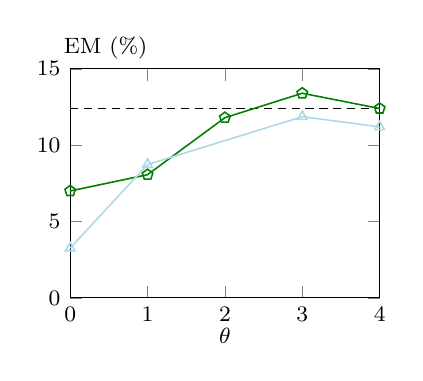
\begin{tikzpicture}[scale=1]
    \begin{axis}[
        height=\columnwidth/2.7,
        width=\columnwidth/2.2,
        ylabel={EM (\%)},
        xlabel={$\theta$},
        xmin=0, xmax=4,
        ymin=0.0, ymax=0.15,
        xtick={0,1,2,3,4},
        xticklabel style = {font=\footnotesize},
        xticklabels={0,1,2,3,4},
        ytick={0, 0.05, 0.10, 0.15},
        yticklabels={0, 5, 10, 15},
        every axis y label/.style={at={(current axis.north west)},right=4.5mm,above=0mm},
        label style={font=\footnotesize},
        tick label style={font=\footnotesize},
        every axis x label/.style={at={(current axis.south)},right=0mm,above=-7mm},
        label style={font=\footnotesize},
        tick label style={font=\footnotesize},
    ]

\addplot[densely dashed, color=black, line width=0.1mm] coordinates {(0, 0.124) (4, 0.124)};
    \addplot[line width=0.2mm,mark size=2pt,mark=o,color=Red]
        plot coordinates { % SkeTRAG

    };

    \addplot[line width=0.2mm,mark size=2pt,mark=pentagon,color=Green]
        plot coordinates { % Hybrid
(0, 0.07)
(1, 0.080666667)
(2, 0.118)
(3, 0.134)
(4, 0.124)
    };

    \addplot[line width=0.2mm,mark size=2pt,mark=triangle,color=LightBlue]
        plot coordinates { % TextRAG
(0, 0.032666667)
(1, 0.087333333)
(3, 0.118666667)
(4, 0.112)
    };
    
    \end{axis}

\end{tikzpicture}

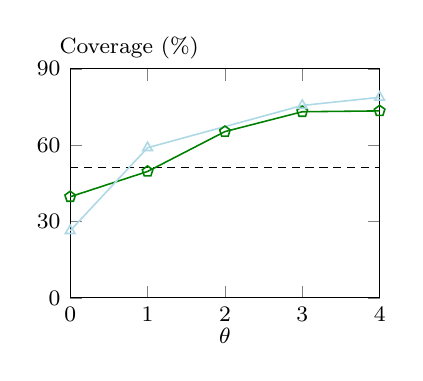
\begin{tikzpicture}[scale=1]
    \begin{axis}[
        height=\columnwidth/2.7,
        width=\columnwidth/2.2,
        ylabel={Coverage (\%)},
        xlabel={$\theta$},
        xmin=0, xmax=4,
        ymin=0.0, ymax=0.9,
        xtick={0,1,2,3,4},
        xticklabel style = {font=\footnotesize},
        xticklabels={0,1,2,3,4},
        ytick={0, 0.3, 0.6, 0.9},
        yticklabels={0, 30, 60, 90},
        every axis y label/.style={at={(current axis.north west)},right=7.5mm,above=0mm},
        label style={font=\footnotesize},
        tick label style={font=\footnotesize},
        every axis x label/.style={at={(current axis.south)},right=0mm,above=-7mm},
        label style={font=\footnotesize},
        tick label style={font=\footnotesize},
    ]

\addplot[densely dashed, color=black, line width=0.1mm] coordinates {(0, 0.514666667
) (4, 0.514666667
)};

    \addplot[line width=0.2mm,mark size=2pt,mark=o,color=Red]
        plot coordinates { % SkeTRAG

    };

    \addplot[line width=0.2mm,mark size=2pt,mark=pentagon,color=Green]
        plot coordinates { % Hybrid
(0, 0.397333333)
(1, 0.496666667)
(2, 0.653333333)
(3, 0.731333333)
(4, 0.734666667)

    };

    \addplot[line width=0.2mm,mark size=2pt,mark=triangle,color=LightBlue]
        plot coordinates { % TextRAG
(0, 0.264)
(1, 0.59)
(3, 0.756)
(4, 0.788)
    };
    
    \end{axis}

\end{tikzpicture}
}%
\caption{Answer quality of PageRank sampling algorithms by varying \#chunk bisections. Dash line represents the performance of GraphRAG.} \label{fig:quality-chunk}
\end{figure}

\subsection{Trade-off Analysis (RQ3)}
In the third set of experiments, we analyze the trade-off between accuracy and cost by varying the budget $\beta$, as well as the balance between the two retrieval channels by adjusting $\theta$. We set $\clen = 150$ and $\tau=0$, and follow the default parameter settings in Section~\ref{sec:exp-set}.

\stitle{Accuracy-cost tradeoff}
Figure~\ref{fig:quality-beta} presents the performance of \sketragu, \sketragp, and \skeletonrag on MuSiQue and HotpotQA by varying $\beta$. 
In particular, \sketragp and \sketragu consistently outperform \skeletonrag, which serves as a lower bound, across different budget $\beta$ values. 
Between the two variants, \sketragp achieves better performance than \sketragu particularly when $\beta\in [0.6, 0.8]$ in MuSiQue and $\beta\in [0.2, 0.4]$ in MuSiQue, demonstrating the effectiveness of identifying core text chunks using PageRank centralities.
Furthermore, the performance of \sketrag is less sensitive to variations in $\beta$ on HotPotQA. For instance, the coverage at $\beta=0.2$ decreases by 2\% compared to $\beta=1$. On MuSiQue, although \sketrag exhibits greater sensitivity in generation quality, its performance quickly catches up once $\beta$ reaches $0.6$. These findings demonstrate \sketrag's effectiveness for further reducing indexing costs.

\stitle{Retrieval channel}
Figure~\ref{fig:quality-theta} reports the performance of \sketragu, \sketragp, and \hybridrag by varying $\theta$.
As illustrated, \sketrag consistently outperforms \hybridrag across different $\theta$ settings, demonstrating the effectiveness of its two key components, \keyrag and \skeletonrag.
Additionally, we observe that the performance of \keyrag improves significantly when incorporating a small fraction (\eg 0.2) of context from \kgrag. This finding further motivates the reduction of costs associated with building a full knowledge graph.
Regarding the two variants, \sketragu and \sketragp, we find that \sketragp achieves superior EM and F1 scores when $\theta \leq 0.4$, which aligns with the trend observed in Figure~\ref{fig:quality-beta}.


\begin{table}[t]
\centering
\renewcommand{\arraystretch}{1.1}
\begin{small}
\caption{Answer quality by varying $\clen$ and $\tau$ on MuSiQue.}
\label{tab:quality-clen}
\begin{tabular}{lcccc|cccc}	
    \toprule
    \bf Param & \multicolumn{4}{c}{\bf $\clen$} & \multicolumn{4}{c}{\bf $\tau$} \\
    \cmidrule(lr){2-5} \cmidrule(lr){6-9}
    \bf Value & \bf 150 & \bf 300 & \bf 600 & \bf 1200 & \bf 3 & \bf 2 & \bf 1 & \bf 0 \\
    \midrule
    \bf Coverage & 79.6 & 79.6 & 77.8 & 77.0 & 77.0 & 70.4 & 61.0 & 56.8 \\
    \bf EM & 19.2 & 18.8 & 15.4 & 14.0 & 14.0 & 13.8 & 11.8 & 12.8\\
    \bf F1 & 22.3 & 18.8 & 17.7 & 17.2 & 18.9 & 18.3 & 16.3 & 17.2\\
    \bottomrule
\end{tabular}
\end{small}
\end{table}

\begin{table}[t]
\centering
\renewcommand{\arraystretch}{1.1}
\begin{small}
\caption{Answer quality by varying $K$ on MuSiQue.}
\label{tab:quality-k}
\begin{tabular}{lccc}	
    \toprule
    \bf $K$ & \bf 2 & \bf 4 & \bf 10\\
    \midrule
    \bf Coverage/EM/F1 & 79.6/19.2/26.1 & 80.0/17.8/25.2 & 80.4/19.4/26.0\\
    \bottomrule
\end{tabular}
\end{small}
\end{table}



\subsection{Parameter Sensitivity (RQ4)}

In the fourth set of experiments, we take the Musique dataset as an example and analyze the sensitivity of \sketragp w.r.t.\ the input text chunk size $\clen$, the number of splits $\tau$, and the integer $K$ used for KNN graph construction.
For $\clen$, we vary $\clen = 150, 300, 600, 1200$ and set the corresponding $\tau = 0, 1, 2, 3$ to maintain a consistent sub-chunk length. For $\tau$, we fix $\clen = 1200$ and vary $\tau = 0, 1, 2, 3$. Additionally, we set $K = 2, 4, 10$ to explore different KNN graph densities.
As shown in Table~\ref{tab:quality-clen}, \sketragp achieves better retrieval and generation quality as the size of input chunks or split sub-chunks decreases. This trend is consistent with the performance of \keyrag and \graphrag in both low- and high-cost settings. These findings align with previous observations~\cite{edge2024local} that smaller chunk sizes improve result quality, further validating the text chunk splitting design in \sketrag. 
Additionally, as shown in Table~\ref{tab:quality-k}, varying the integer $K$ from 2 to 10 results in only minor changes in coverage, EM, and F1 scores, \eg 79.6/19.2/26.1 for $K = 2$ vs.\ 80.4/19.4/26.0 for $K = 10$, indicating that \sketrag is not significantly affected by the density of the KNN graph. This stability can be explained by Figure \ref{fig:degree-distribution}, which shows that KNN graphs with different $K$ exhibit similar degree distribution shapes, despite variations in average degree.